\documentclass[a4paper,14pt]{extarticle}

% Путь до папки с общими шаблонами
\newcommand{\pathToCommonFolder}{/home/denilai/Desktop/LaTeX/Common}
% Название работы в титуле
\newcommand{\workname}{Отчет по практической работе №4}
% Название дисциплины в титуле
\newcommand{\discipline}{Системное программное обеспечение}
% Название кафедры в титуле
\newcommand{\kafedra}{Кафедра Математического обеспечения и стандартизации информационных технологий}
% Тема работы в титуле
\newcommand{\theme}{Системы конфигурационного управления}
\newcommand{\rang}{ассистент}
\newcommand{\teacherfio}{Ю.~А.~Вороноцов}



% установка размера шрифта для всего документа
%\fontsize{20pt}{18pt}\selectfont
\usepackage{extsizes} % Возможность сделать 14-й шрифт

\author{Кирилл Денисов}
\title{Практическая работа №3}
\date{\today}

% установка полуторного интервала
% \usepackage{setspace}  
% \onehalfspacing



% Вставка заготовки преамбулы
% Этот шаблон документа разработан в 2014 году
% Данилом Фёдоровых (danil@fedorovykh.ru) 
% для использования в курсе 
% <<Документы и презентации в \LaTeX>>, записанном НИУ ВШЭ
% для Coursera.org: http://coursera.org/course/latex .
% Исходная версия шаблона --- 
% https://www.writelatex.com/coursera/latex/5.3

% В этом документе преамбула

% Для корректного использования русских символов в формулах
% пакеты hyperref и настройки, связанные с ним, стоит загуржать
% перед загрузкой пакета mathtext



% поддержка русских букв
% кодировка шрифта
%\usepackage[T2A]{fontenc} 
\usepackage{pscyr}

% использование ненумеровонного абзаца с добавлением его в содержаниеl

\newcommand{\anonsection}[1]{\section*{#1}\addcontentsline{toc}{section}{#1}}
\newcommand{\sectionunderl}[1]{\section*{\underline{#1}}}


% настройка окружения enumerate
\usepackage{enumitem}
\setlist{noitemsep}
\setlist[enumerate]{labelsep=*, leftmargin=1.5pc}

\usepackage{hyperref}

% сначала ставить \usepackage{extsizes} % Возможность сделать 14-й шрифт
% для корректной установки полей вставлять преамбулу следует в последнюю очередь (но перед дерективой замены \rmdefault)
\usepackage[top=20mm,bottom=25mm,left=35mm,right=20mm]{geometry} % Простой способ задавать поля

\hypersetup{				% Гиперссылки
	unicode=true,           % русские буквы в раздела PDF
	pdftitle={Заголовок},   % Заголовок
	pdfauthor={Автор},      % Автор
	pdfsubject={Тема},      % Тема
	pdfcreator={Создатель}, % Создатель
	pdfproducer={Производитель}, % Производитель
	pdfkeywords={keyword1} {key2} {key3}, % Ключевые слова
	colorlinks=true,       	% false: ссылки в рамках; true: цветные ссылки
	linkcolor=red,          % внутренние ссылки
	citecolor=black,        % на библиографию
	filecolor=magenta,      % на файлы
	urlcolor=blue           % на URL
}

%%% Работа с русским языком
\usepackage{cmap}					% поиск в PDF
\usepackage{mathtext} 				% русские буквы в формулах
\usepackage[T2A]{fontenc}			% кодировка
\usepackage[utf8]{inputenc}			% кодировка исходного текста
\usepackage[english,russian]{babel}	% локализация и переносы
\usepackage{indentfirst}
\frenchspacing

%для изменения названия списка иллюстраций
\usepackage{tocloft}


\renewcommand{\epsilon}{\ensuremath{\varepsilon}}
\renewcommand{\phi}{\ensuremath{\varphi}}
\renewcommand{\kappa}{\ensuremath{\varkappa}}
\renewcommand{\le}{\ensuremath{\leqslant}}
\renewcommand{\leq}{\ensuremath{\leqslant}}
\renewcommand{\ge}{\ensuremath{\geqslant}}
\renewcommand{\geq}{\ensuremath{\geqslant}}
\renewcommand{\emptyset}{\varnothing}

% Изменения параметров списка иллюстраций
\renewcommand{\cftfigfont}{Рисунок } % добавляем везде "Рисунок" перед номером
\addto\captionsrussian{\renewcommand\listfigurename{Список иллюстративного материала}}

\newcommand{\tm}{\texttrademark\ }
\newcommand{\reg}{\textregistered\ }


%%% Дополнительная работа с математикой
\usepackage{amsmath,amsfonts,amssymb,amsthm,mathtools} % AMS
\usepackage{icomma} % "Умная" запятая: $0,2$ --- число, $0, 2$ --- перечисление

%% Номера формул
%\mathtoolsset{showonlyrefs=true} % Показывать номера только у тех формул, на которые есть \eqref{} в тексте.
%\usepackage{leqno} % Нумереация формул слева

%% Свои команды
\DeclareMathOperator{\sgn}{\mathop{sgn}}

%% Перенос знаков в формулах (по Львовскому)
\newcommand*{\hm}[1]{#1\nobreak\discretionary{}
{\hbox{$\mathsurround=0pt #1$}}{}}


% отступ для первого абзаца главы или параграфа
%\usepackage{indentfirst}

%%% Работа с картинками
\usepackage{graphicx}  % Для вставки рисунков
\graphicspath{{images/}{screnshots/}}  % папки с картинками
\DeclareGraphicsExtensions{.pdf,.png,.jpg}
\setlength\fboxsep{3pt} % Отступ рамки \fbox{} от рисунка
\setlength\fboxrule{1pt} % Толщина линий рамки \fbox{}
\usepackage{wrapfig} % Обтекание рисунков текстом

%%% Работа с таблицами
\usepackage{array,tabularx,tabulary,booktabs} % Дополнительная работа с таблицами
\usepackage{longtable}  % Длинные таблицы
\usepackage{multirow} % Слияние строк в таблице

%%% Теоремы
\theoremstyle{plain} % Это стиль по умолчанию, его можно не переопределять.
\newtheorem{theorem}{Теорема}[section]
\newtheorem{proposition}[theorem]{Утверждение}

\theoremstyle{plain} % Это стиль по умолчанию, его можно не переопределять.
\newtheorem{work}{Практическая работа}[part]


 
 
\theoremstyle{definition} % "Определение"
\newtheorem{corollary}{Следствие}[theorem]
\newtheorem{problem}{Задача}[section]
 
\theoremstyle{remark} % "Примечание"
\newtheorem*{nonum}{Решение}



%%% Программирование
\usepackage{etoolbox} % логические операторы

%%% Страница

%	\usepackage{fancyhdr} % Колонтитулы
% 	\pagestyle{fancy}
%   \renewcommand{\headrulewidth}{0pt}  % Толщина линейки, отчеркивающей верхний колонтитул
% 	\lfoot{Нижний левый}
% 	\rfoot{Нижний правый}
% 	\rhead{Верхний правый}
% 	\chead{Верхний в центре}
% 	\lhead{Верхний левый}
%	\cfoot{Нижний в центре} % По умолчанию здесь номер страницы

\usepackage{setspace} % Интерлиньяж
\onehalfspacing % Интерлиньяж 1.5
%\doublespacing % Интерлиньяж 2
%\singlespacing % Интерлиньяж 1

\usepackage{lastpage} % Узнать, сколько всего страниц в документе.

\usepackage{soul} % Модификаторы начертания


\usepackage[usenames,dvipsnames,svgnames,table,rgb]{xcolor}


\usepackage{csquotes} % Еще инструменты для ссылок

%\usepackage[style=authoryear,maxcitenames=2,backend=biber,sorting=nty]{biblatex}

\usepackage{multicol} % Несколько колонок

\usepackage{tikz} % Работа с графикой
\usepackage{pgfplots}
\usepackage{pgfplotstable}

% модуль для вставки рыбы
\usepackage{blindtext}

\usepackage{listings}
\usepackage{color}


% для поворота отдельной страницы. Использовать окружение \landscape
\usepackage{pdflscape} 
\usepackage{rotating} 


\definecolor{mygreen}{rgb}{0,0.6,0}
\definecolor{mygray}{rgb}{0.5,0.5,0.5}
\definecolor{mymauve}{rgb}{0.58,0,0.82}


% пример импорта файла
%\lstinputlisting{/home/denilai/repomy/conf/distributions}

\lstset{
	language=Python,
	basicstyle=\footnotesize,        % the size of the fonts that are used for the code
	numbers=left,                    % where to put the line-numbers; possible values are (none, left, right)
	numbersep=5pt,                   % how far the line-numbers are from the code
	numberstyle=\tiny\color{mygray}, % the style that is used for the line-numbers
	stepnumber=2,                    % the step between two line-numbers. If it's 1, each line will be numbered
	% Tab - 2 пробела
	tabsize=2,    
	% Автоматический перенос строк
	breaklines=true,
	frame=single,
	breakatwhitespace=true,
	title=\lstname 
}



% использовать Times New Roman
\renewcommand{\rmdefault}{ftm}

\begin{document}
	\thispagestyle{empty}
	
	% Вставка первого титульного листа
	%\newcounter{withouttheme}

%\setcounter{withouttheme}{<n>} установить значение счетчика  withouttheme для определения, нужна ли тема
%    {0} - нужна
%    {1} - не нужна

%\setcounter{withoutsubmissiondate}{<n>} установить значение счетчика  withoutsubmissiondate для определения, нужна ли дата представления к защите
%     {0} - нужна
%     {1} - не нужена
\begin{center}
	\begin{figure}[h!]
		\begin{center}
		%\vspace{-10ex}
		
\includegraphics[width=0.17\linewidth]{\pathToCommonFolder/gerb}
		%\caption{}\label{pic:first}
		%	\vspace{5ex}
		\end{center}	
	\end{figure}
 	\small	МИНОБРНАУКИ РОССИИ \\
	Федеральное государственное бюджетное образовательное учреждение\\
						высшего образования\\
\normalsize					
\textbf{«МИРЭА – Российский технологический университет»\\
						РТУ МИРЭА}\\
						\noindent\rule{1\linewidth}{1pt}\\
       Институт информационных технологий\\ %\vspace{2ex}
					\kafedra\\
		\vspace{3ex}
			\large \textbf{\workname}  \\
		%\vspace{1ex}
						по дисциплине\\ «\discipline» \\
		\vspace{3ex}
		\ifnum \value{withouttheme}=0 {
			\textbf{Тема работы:}\\ <<\theme>>
		}
		\else {}
		\fi
\vspace{10ex}
\small
\begin{table}[h!]
\begin{tabular}{lp{0.6\linewidth}l}
	\textbf{Выполнил:} & студент группы ИВБО-02-19 & \\ 
	& & \studentfio \\%Д.~Н.~Федосеев\\%А.~М.~Сосунов\\%К.~Ю.~Денисов\\%И.~А.~Кремнев
	\textbf{Принял:} & \rang & \\
	& & \teacherfio \hfill\\
\end{tabular}
\end{table}
\end{center}
\ifnum \value{withoutsubmissiondate}=0 {
	\begin{flushleft}
		Работа представлена к защите <<\rule{3ex}{1pt}>>\rule{10ex}{1pt} 202\rule{1ex}{1pt} г.\hfill
	\end{flushleft}
\else {}
\fi

\normalsize
\begin{center}	
\vfill
Москва 2022
\end{center}

	
	\newpage
	\tableofcontents
	\newpage

\section{Образы}
С помощью данных команд проверим имеющиеся образы и контейнеры docker, загрузим образ ubuntu.
\begin{lstlisting}
	$ docker images
	$ docker ps -a
	$ docker pull ubuntu
\end{lstlisting}


\section {Изоляция}
Приведем ответ на вопрос \textit{"Одинаковый ли результат получился при разных запусках?"}

При выполнении данной команды на локальной машине ответ ожидаемо один и тот же, но при выполнении данной команды в контейнере Docker, каждый раз ответ отличался. Это связано с тем, что из одного образа ubuntu были запущены два изолированных контейнера, поэтому у них и был разный hostname.

Запуск контейнеров производится командой:
\begin{lstlisting}
	$ docker run --flags --docker container_name commsnds -and --boot --flags --program
\end{lstlisting}

Запустим bash с возможностью входа в интерактивную оболочку, используя флаги \texttt{-if}:
\begin{lstlisting}
$ docker run -it ubuntu bash.
\end{lstlisting}

Результаты выполнения команд  пунктов 1 и 2 можно увидеть на рисунке \ref{img:1and2} \hyperref[A]{Приложении А}.



\section{Работа с портами}
Загрузим образ \texttt{python} командой \texttt{docker pull python}. Запустим модуль веб-сервера из корня контейнера, чтобы отобразить содержание контейнера с помощью команд.
\begin{lstlisting}
  $ docker pull python
  $ docker run -it python python m http.server
\end{lstlisting}

ля проброса портов используется флаг \texttt{-p hostPort:containerPort}.
Для того, чтобы доступный в контейнере на порту 8000 веб-сайт в хостовой системе открывался на
порту 8888, необходимо указать флаг \texttt{-p 8888:8000}.

\begin{lstlisting}
$ docker run -it -p8000:8000 python python -m http.server
\end{lstlisting}

\section{Именованные контейнеры, остановка и удаление}
Запустим контейнер в фоне, используя флаг \texttt{--d}, указав имя для него с помощью флага \texttt{--name}. После запуска контейнера можно удалить его, предварительно остановив используя команду \texttt{docker stop <name>}. 
Для того, чтобы контейнер удалялся после завершения работы, нужно указать флаг \texttt{--rm} при его
запуске — далее в работе мы будем использовать данный флаг. Приведем команды, используемые в данном пункте:
\begin{lstlisting}
	$ docker run --rm -p8000:8000 --name pyserver -d python python -m http.server
	$ docker stop pyserver
\end{lstlisting}
Результаты выполнения команд из пунктов 3 и 4 можно увидеть на рис. \ref{img:3and4} и \ref{img:4file} в \hyperref[A]{Приложении А}.

\section{Постоянное хранение данных}
Для того, чтобы иметь возможность сохранять результаты работы приложения в файлах, используем флаг \texttt{-d} после указания названия образа, который указывает модулю \texttt{http.server} какая директория будет корневой для отображения.

Выполним команду:
\begin{lstlisting}
    $ docker run -p8000:8000 --name pyserver --rm -d python python -m http.server -d /mnt
\end{lstlisting}

После выполнения данной команды запустим оболочку bash и создадим файл \textit{hi.txt}, в который поместим строку \textit{"hello world"}. Если Если открыть http://0.0.0.0:8000/, там будет доступен файл hi.txt.

После остановки контейнера и повторного запуска данный файл больше не будет доступен. Так как мы запустили новый контейнер, а старый вместе со всеми файлами, созданными им, был удален после завершения работы.

Для того, чтобы не терялись какие-то данные (например, если запущен контейнер с СУБД, то чтобы
не терялись данные из неё) существует механизм монтирования.

Приведем ответ на вопрос \textit{"Что значат остальные флаги запуска? Где здесь команда, которая выполнится в контейнере?"}
\begin{itemize}
	\item \texttt{-\,-name} позволяет задавать имя для контейнера;
	\item \texttt{-\,-rm} удалять контейнер после остановки;
	\item \texttt{-d} перед названием образа позволяет запускать контейнер в фоновом режиме;
	\item \texttt{-m} позволяет запустить модуль из корня контейнера;
	\item \texttt{-d} в конце указывает на то, какая директория будет корневой для отображения.
\end{itemize}

Команда, которая выполнится в контейнере --- \texttt{python -m http.server -d /mnt}.

Результаты выполнения перечисленных команд можно увидеть на рис. \ref{img:5com} и \ref{img:5serv} в \hyperref[A]{Приложении А}.

\subsection{Тома}

Первый способ — это создать отдельный том с помощью ключа \texttt{-v myvolume:/mnt}, где \texttt{myvolume} —
название тома, \texttt{/mnt} — директория в контейнере, где будут доступны данные.

Воспользуемся командой:
\begin{lstlisting}
 $ docker run -p8000:8000 --rm --name pyserver -d -v $ ( pwd )/ myfiles :/ mnt python python -m http.server -d /mnt
\end{lstlisting}

Затем, если создать файл (выполнить \texttt{docker exec -it pyserver bash} и внутри контейнера выполнить \texttt{cd mnt \&\& echo "hello world" > hi.txt)}, то даже после удаления контейнера данные в этом томе будут сохранены.

Чтобы узнать где хранятся данные, выполните команду
\texttt{docker inspect -f "{{json .Mounts }}" pyserver}, в поле Source будет храниться путь до тома на
хостовой машине. См. рис. \ref{img:5.1.1} и \ref{img:5.1.2} в \hyperref[A]{Приложении А}.

\subsection{Монтрирование директорий и файлов}

Иногда требуется пробросить в контейнер конфигурационный файл или отдельную директорию. Для
этого используется монтирование директорий и файлов.
Создадим директорию и файлы, которые будем монтировать. Часть из них нам понадобится дальше:
создадим директорию: \texttt{mkdir myfiles}, в ней создадим файл \textit{host.txt:} \texttt{touch myfiles/host.txt}
Запустим контейнер:
\begin{lstlisting}
	$ docker run -p8000:8000 --rm --name pyserver -d -v (pwd)/myfiles:/mnt python python -m http.server -d /mnt
	

\end{lstlisting} 
	Затем, перейдем в контейнер: \texttt{docker exec -it pyserver bash}, перейдем в директорию \textit{mnt} командой
\texttt{cd /mnt}. Если вывести список файлов командой \texttt{ls}, то там будет файл \textit{host.txt}, примонтированный
вместе с директорией \textit{myfiles}.


\section{Переменные окружения}
Для передачи переменных окружения внутрь контейнера используется ключ \texttt{-e}. Например, чтобы
передать в контейнер переменную окружения \textit{MIREA} cо значением \textit{<<ONE LOVE>>}, нужно добавить
ключ \texttt{-e MIREA="ONE LOVE"}.
Проверим, выведя все переменные окружения, определённые в контейнере с помощью утилиты \textit{env:}
\begin{lstlisting}
	$docker run -it --rm -e MIREA="ONE LOVE" ubuntu env
\end{lstlisting}
Среди списка переменных будет и MIREA. См. рис. \ref{img:6}.

\section{Dockerfile}

Соберем образ, в который будут установлены дополнительные пакеты, примонтируем директорию и установим команду запуска. Для этого создадим файл \textit{Dockerfile}.

\lstinputlisting{/home/denilai/gg/Dockerfile}
\begin{itemize}
	\item В строке (1) указывается базовый образ, на основе которого будет строиться новый образ.
	\item В строках (2-5) указана команда, которая выполнится в процессе сборки. На самом деле, там выпол-
няются несколько команд, соединённых \&\& для того, чтобы создавать меньше слоёв в образе.
	\item В строках (6) тоже указана команда, которая сгенерирует случайную цитату и перенаправит вывод в
файл /mnt/greeting-while-building.txt. Файл будет сгенерирован во время сборки образа.
	\item В строке (7) копируется всё содержимое директории ./data хостовой машины в директорию /mnt,
которая будет доступна в контейнере.
	\item В строке (8) указывается, какой порт у контейнера будет открыт.
	\item В строке (9) указывается команда, которая будет выполнена при запуске, где 80 — порт, который будет
слушать веб-сервер.
\end{itemize}

Соберем образ с тегом \textit{mycoolimage} с помощью команды \texttt{docker build -t mycoolimage .}

Точка в
конце указывает на текущую директорию, где лежит Dockerfile.
Запуск производится командой \texttt{docker run --rm -it -p8099:80 mycoolimage}, где порт 8099 — порт на хостовой машине.

Результаты создания образа, запуска контейнера и обращения к серверу можно видеть на рисунках \ref{img:7com}, \ref{img:7serv} и \ref{img:7file} в \hyperref[A]{Приложении А}.

\section{Индивидуальное задание}
В качестве индивидуального задания предложено написать Dockerfile, собрать образ, запустить контейнер (и записать команду для его запуска). 

Для монтирования создайте директорию data и в ней файл \textit{student.txt}, содержащий ФИО, название группы и номер варианта.

Условия согласно варианту:
\begin{itemize}
	\item необходимо использовать базовый образ ubuntu:20.10;
	\item примонтировать файл data/student.txt как /mnt/files/student.txt в контейнере;
	\item установить пакет patch.
\end{itemize}

Запустить веб-сервер, отображающий содержимое /mnt/files, в хостовой системе должен открываться на порту (8800 + номер варианта). Например, для 22-го варианта это порт 8822.

Приведем содержание Dockerfile, который создает образ согласно вышеизложенным требованиям. 

\lstinputlisting{/home/denilai/data/Dockerfile}

Для сборки образа используем команду

\begin{lstlisting}
$ docker build -t myvariant .
\end{lstlisting}

Для запуска контейнера по данному образу используем команду 

\begin{lstlisting}
$docker run --rm -it -p8806:80 -v \$(pwd)/student.txt:/mnt/files/student.txt myvariant
\end{lstlisting}

Результаты выполнения команд и открытие файлов на сервере можно увидеть на рисунках \ref{img:8com}, \ref{img:8serv}, \ref{img:8serv1} и \ref{img:8file} в \hyperref[A]{Приложении А}.

\section{Вывод}
В ходе данной практической работы мы познакомились с командами по созданию Docker-образов, Docker-контейнеров, научились монтировать директории и отдельные файлы в контейнер, пробрасывать переменные окружения, настраивать внутренние и внешние порты, познакомились и разобрали структуру Dockerfile.

Применили все полученные знания для создания собственного образа и контейнера.
\newpage
{\centering
\anonsection{ПРИЛОЖЕНИЕ А}
}
\label{A}
\begin{figure}[hptb]
	\centering
	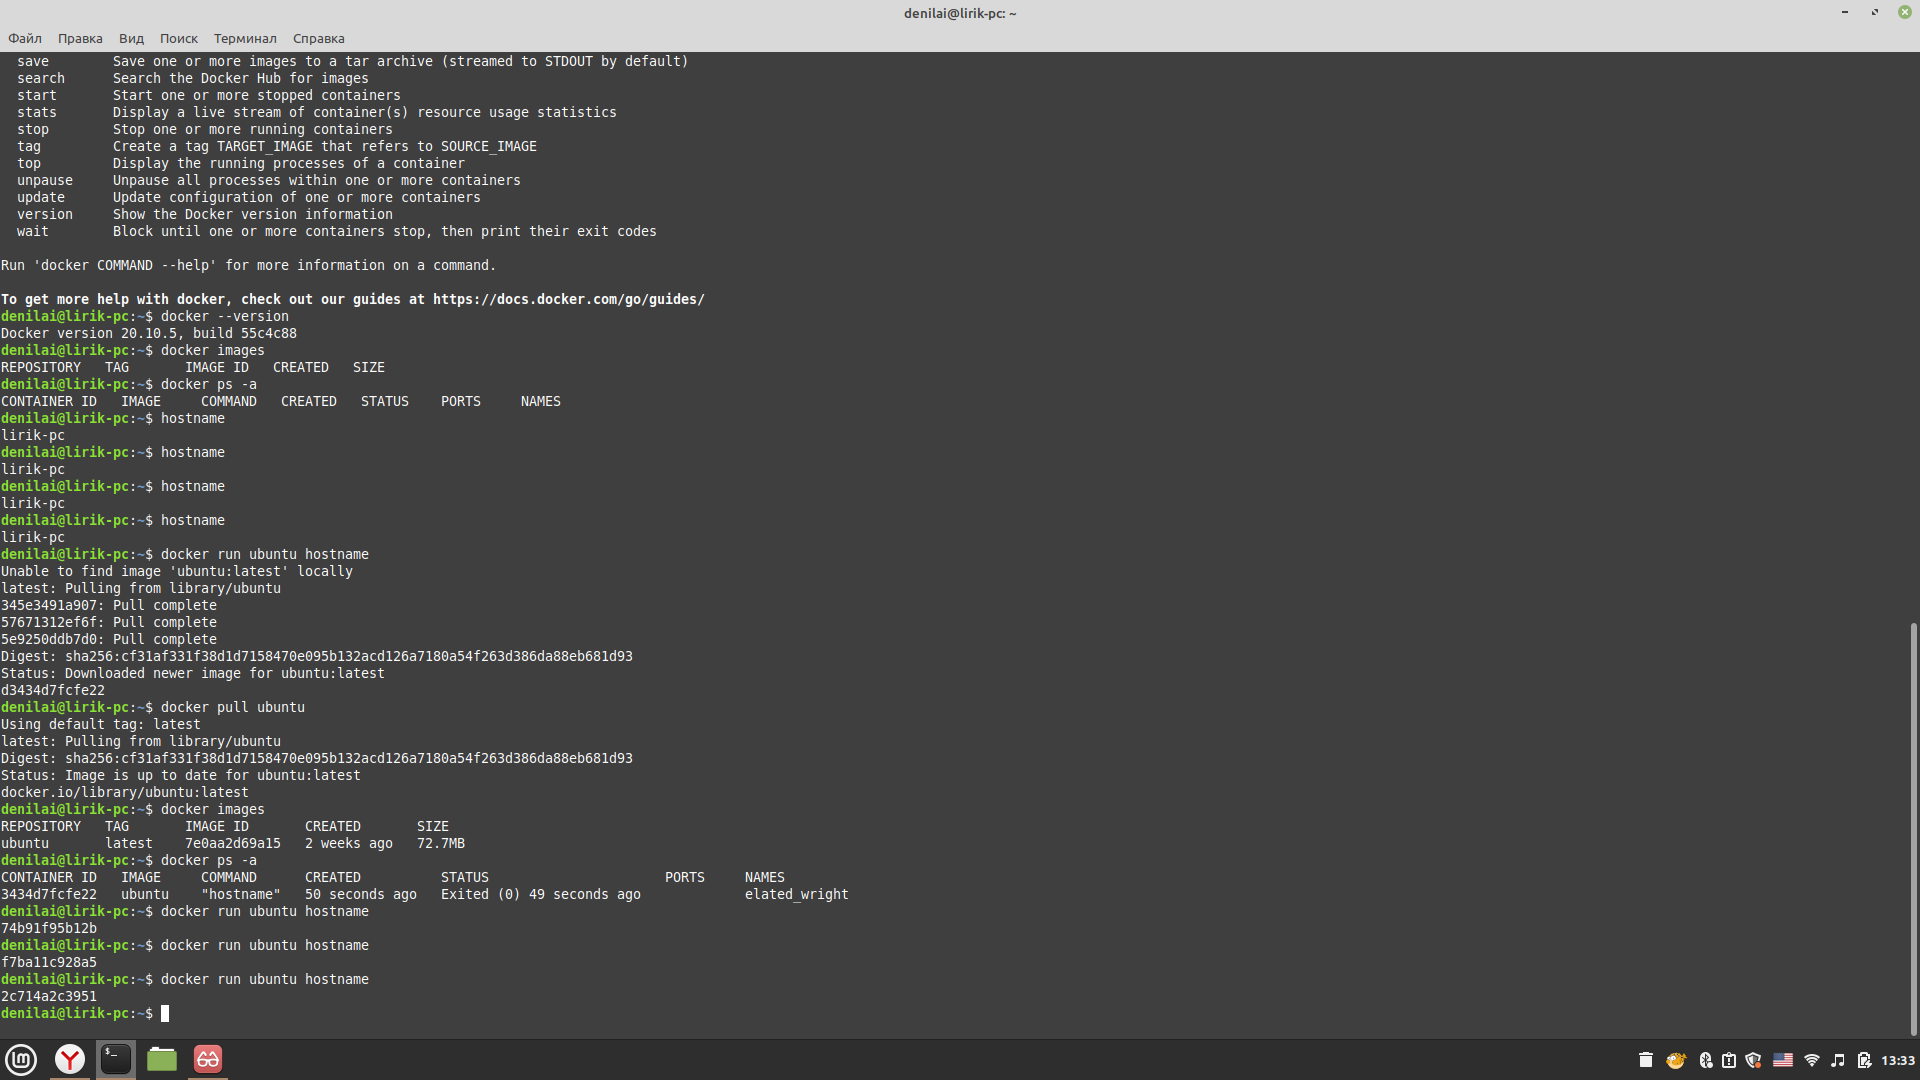
\includegraphics[width=\linewidth]{1and2}
	\caption{Образы и изоляция}
	\label{img:1and2}
\end{figure}

\begin{figure}[hptb]
	\centering
	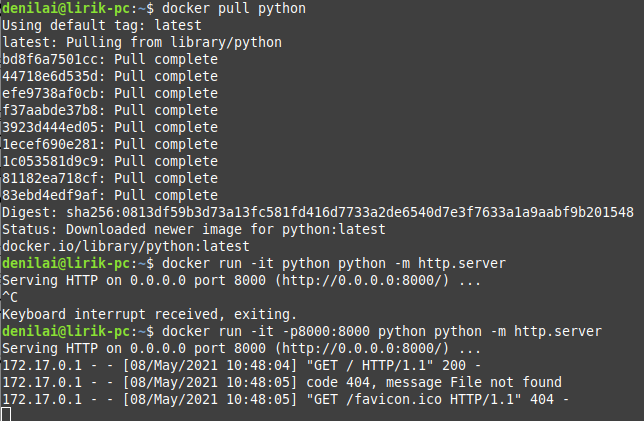
\includegraphics[width=\linewidth]{3}
	\caption{Работа с портами}
	\label{img:3and4}
\end{figure}

\begin{figure}[hptb]
	\centering
	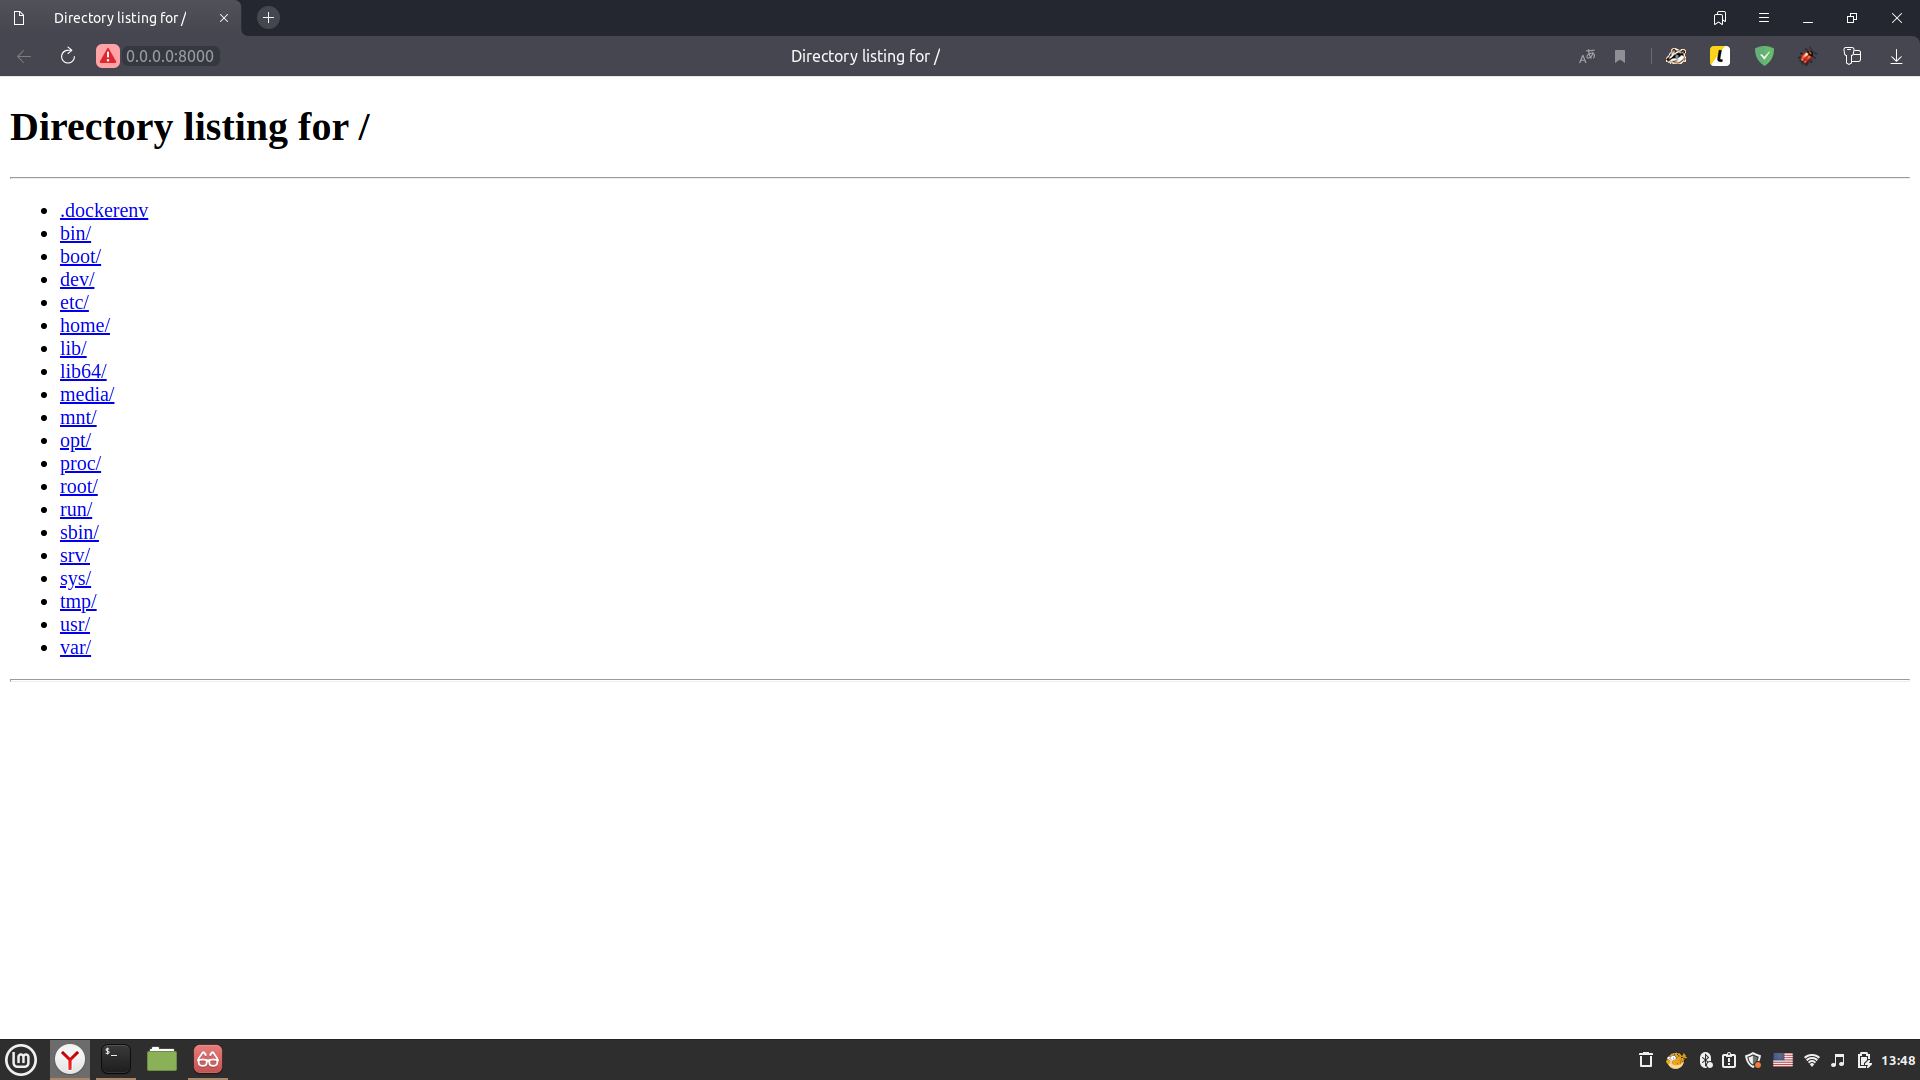
\includegraphics[width=\linewidth]{3serv}
	\caption{Работа с портами. Веб-сервер}
	\label{img:3serv}
\end{figure}

\begin{figure}[hptb]
	\centering
	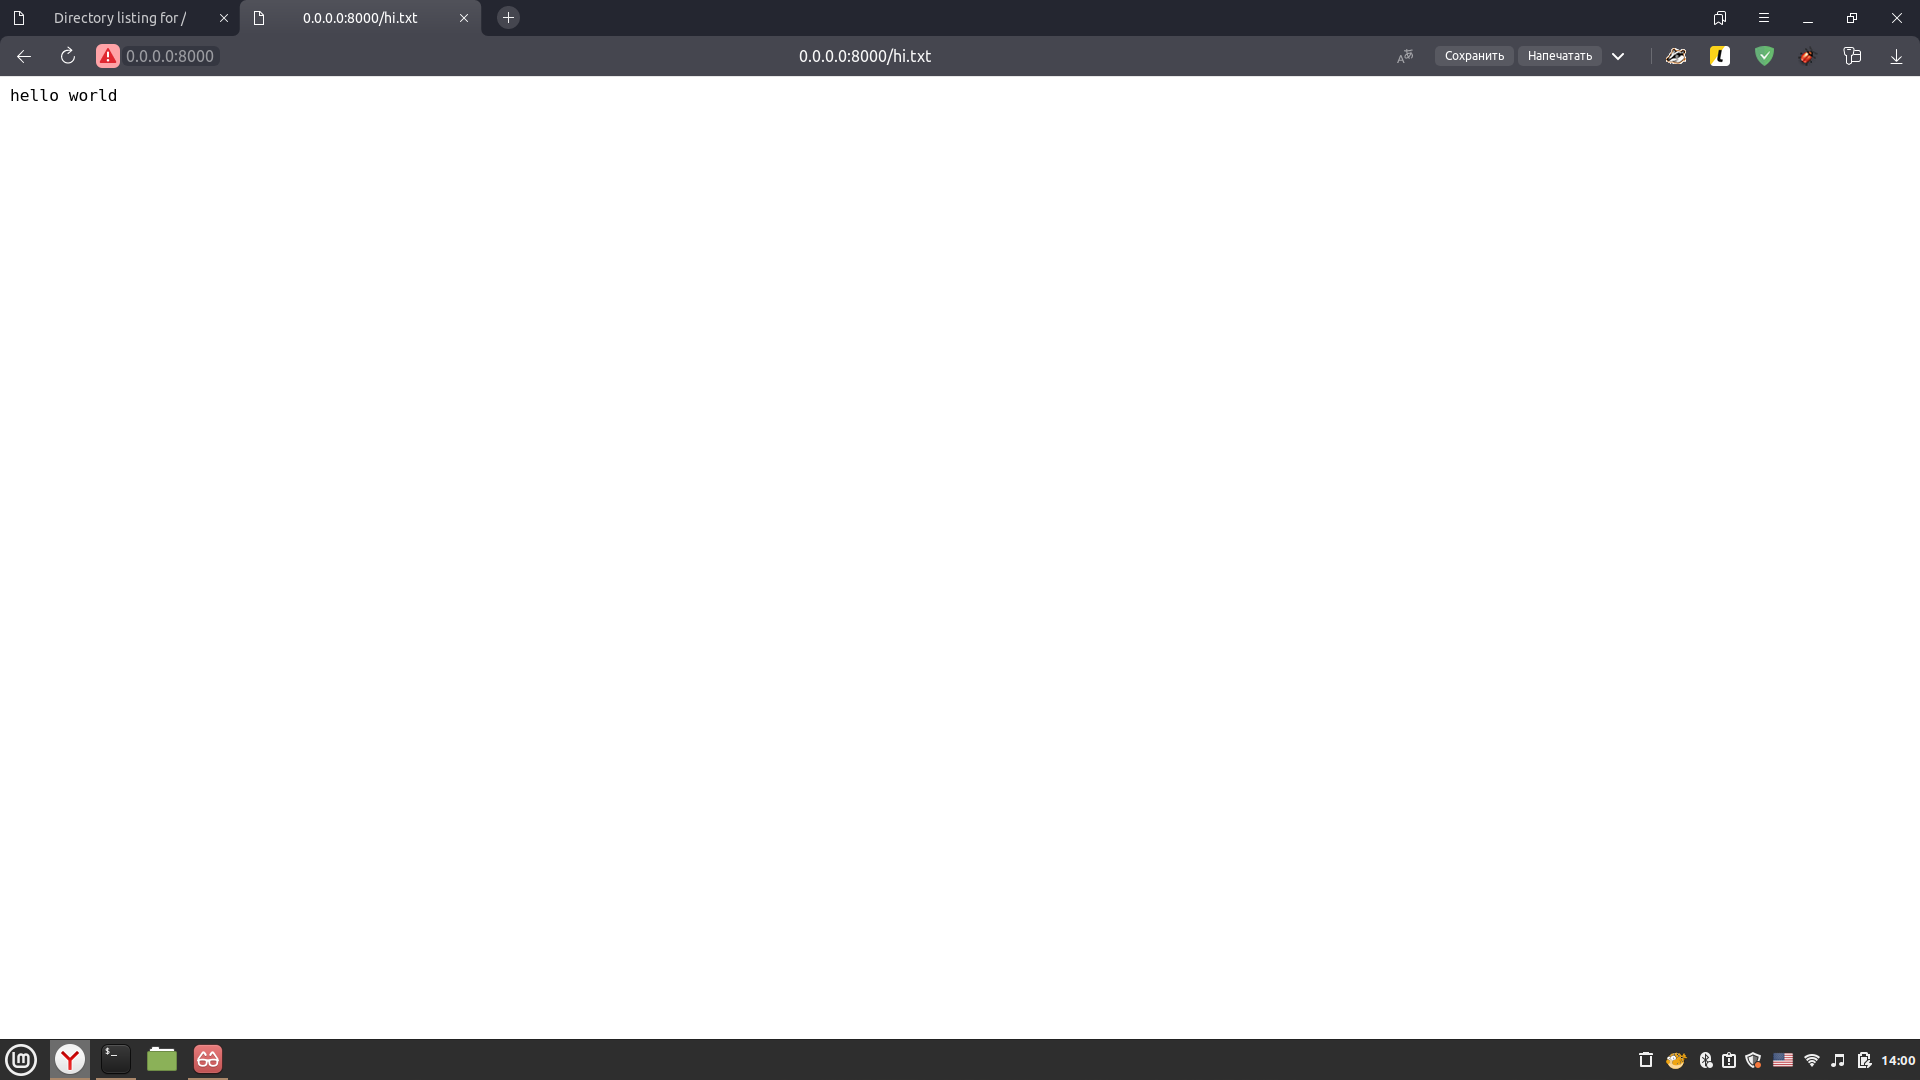
\includegraphics[width=\linewidth]{4file}
	\caption{Работа с портами. Файл}
	\label{img:4file}
\end{figure}
\newpage
\begin{figure}[hptb]
	\centering
	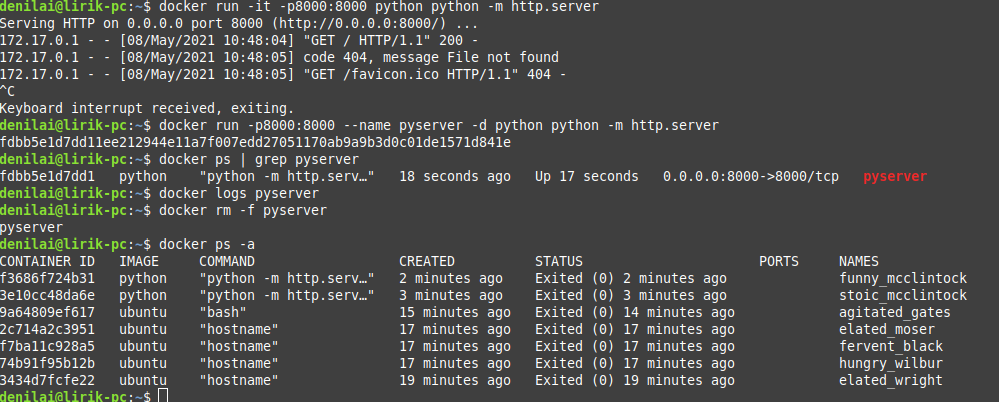
\includegraphics[width=\linewidth]{5com}
	\caption{Постоянное хранение}
	\label{img:5com}
\end{figure}
\newpage
\begin{figure}[hptb]
	\centering
	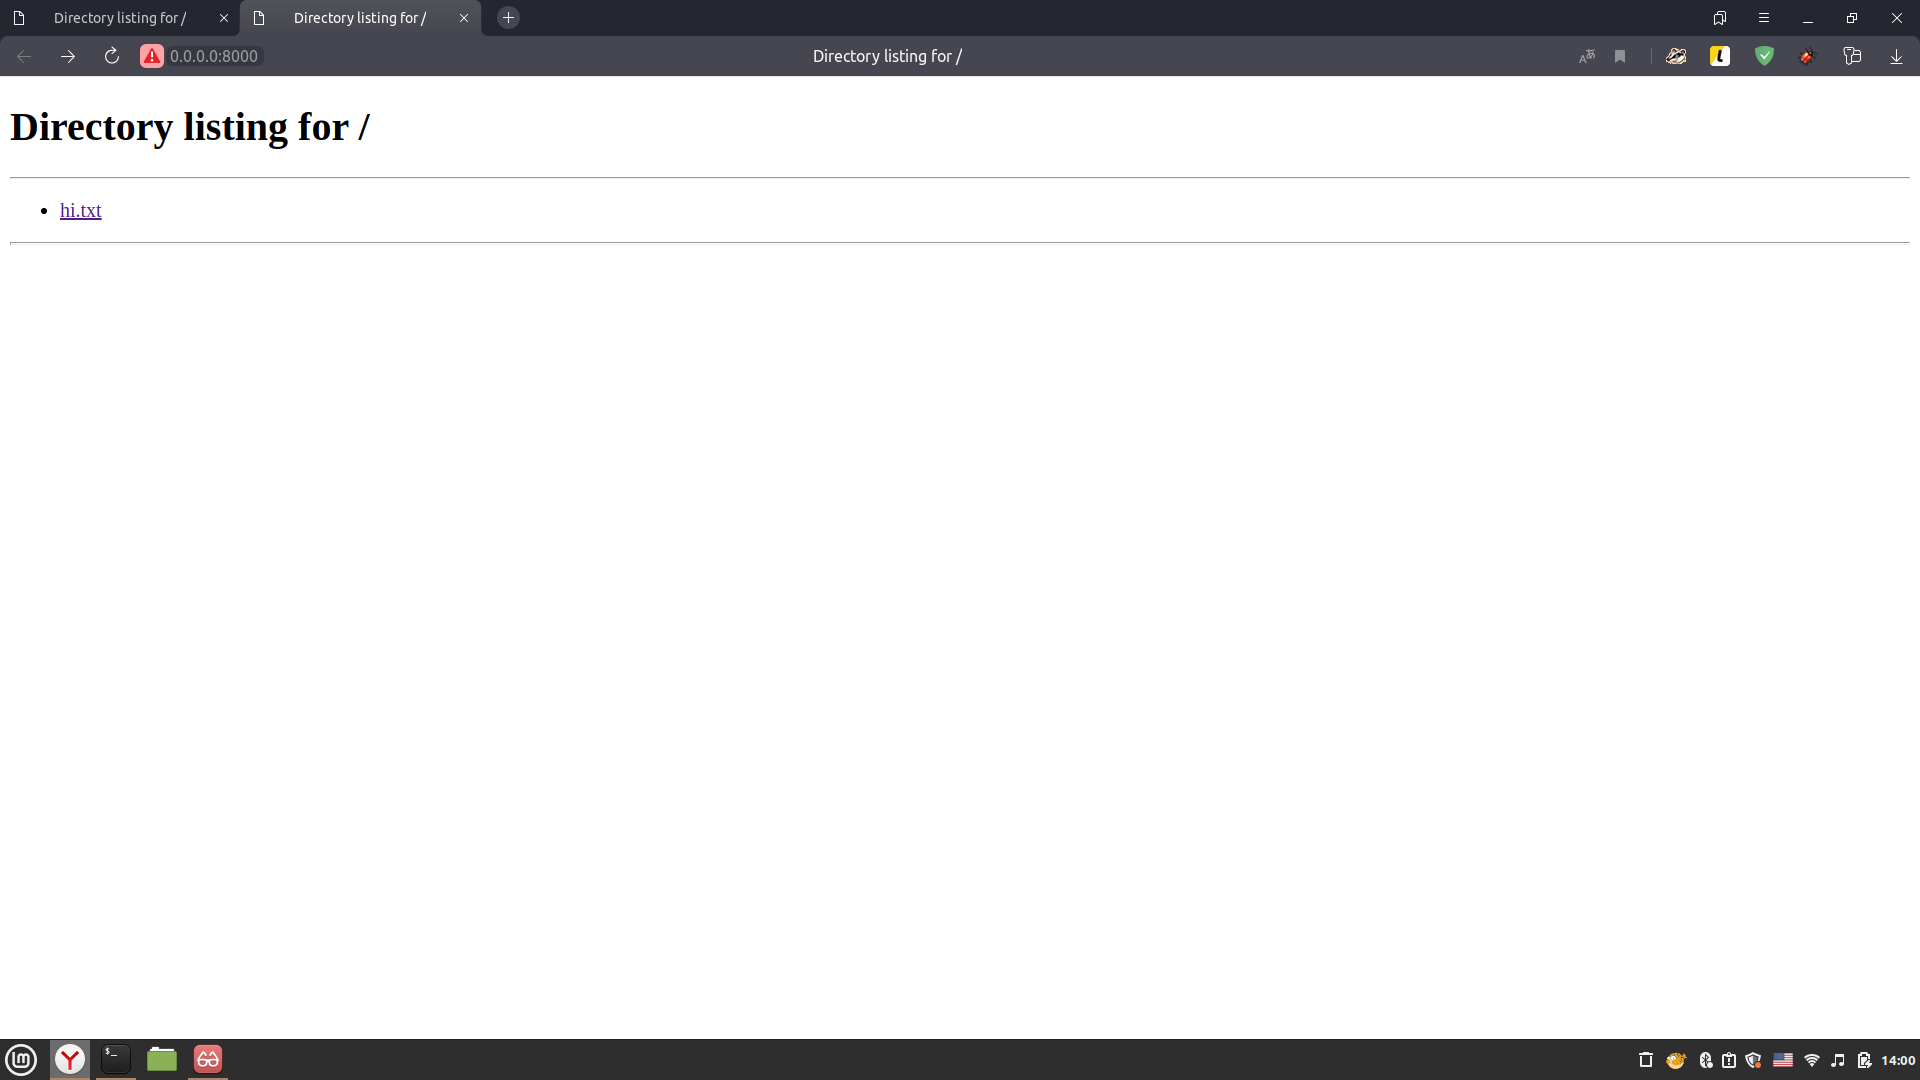
\includegraphics[width=\linewidth]{5serv}
	\caption{Постоянное хранение. Веб-сервер}
	\label{img:5serv}
\end{figure}

\begin{figure}[hptb]
	\centering
	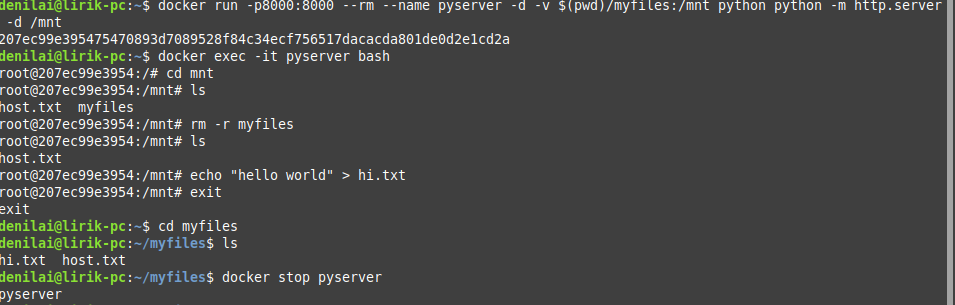
\includegraphics[width=\linewidth]{5.1.1}
	\caption{Тома}
	\label{img:5.1.1}
\end{figure}

\begin{figure}[hptb]
	\centering
	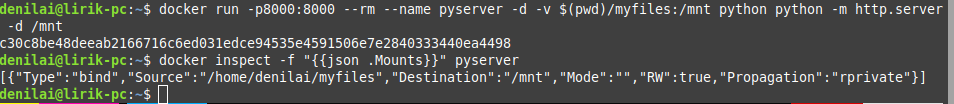
\includegraphics[width=\linewidth]{5.1.2}
	\caption{Тома. Локальное место хранения}
	\label{img:5.1.2}
\end{figure}

\begin{figure}[hptb]
	\centering
	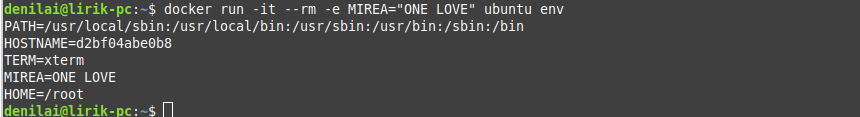
\includegraphics[width=\linewidth]{6}
	\caption{Переменные окружения}
	\label{img:6}
\end{figure}

\begin{figure}[hptb]
	\centering
	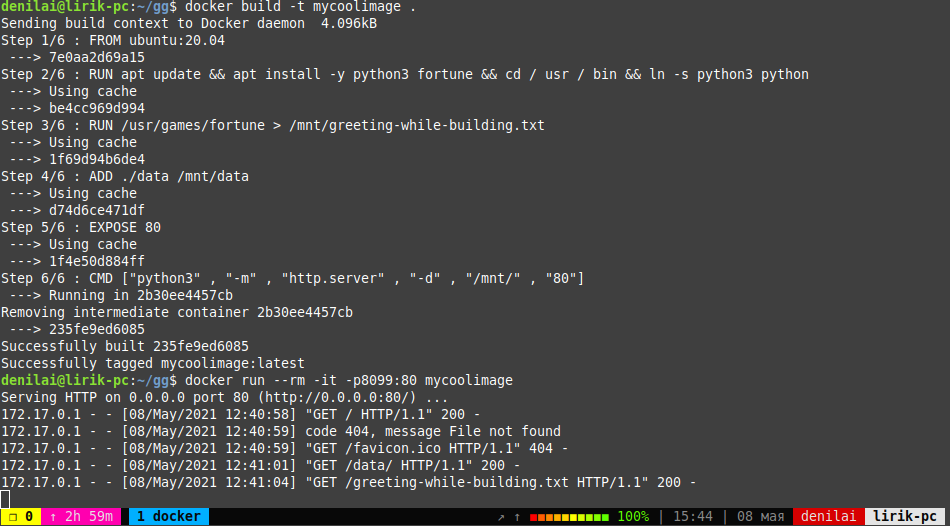
\includegraphics[width=\linewidth]{7com}
	\caption{Dockerfile. Команды}
	\label{img:7com}
\end{figure}


\begin{figure}[hptb]
	\centering
	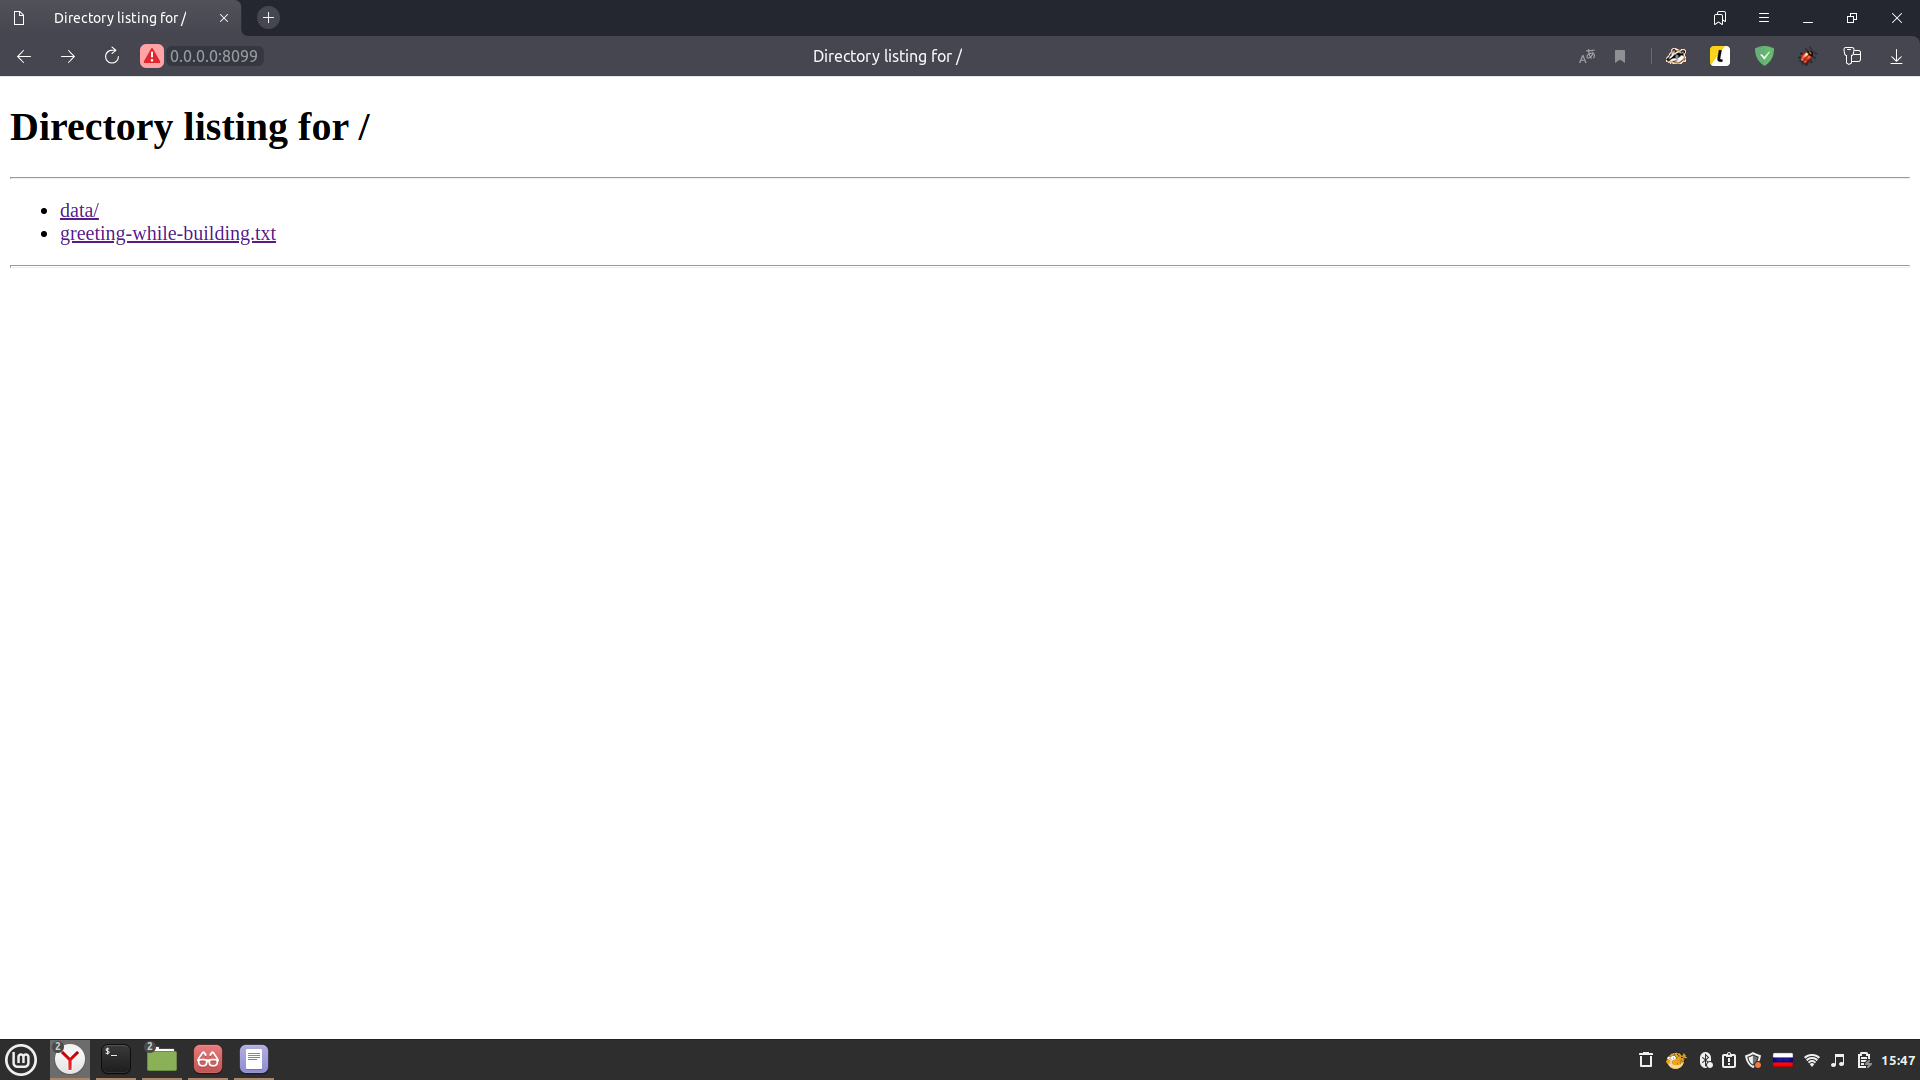
\includegraphics[width=\linewidth]{7serv}
	\caption{Dockerfile. Сервер}
	\label{img:7serv}
\end{figure}

\newpage
\begin{figure}[hptb]
	\centering
	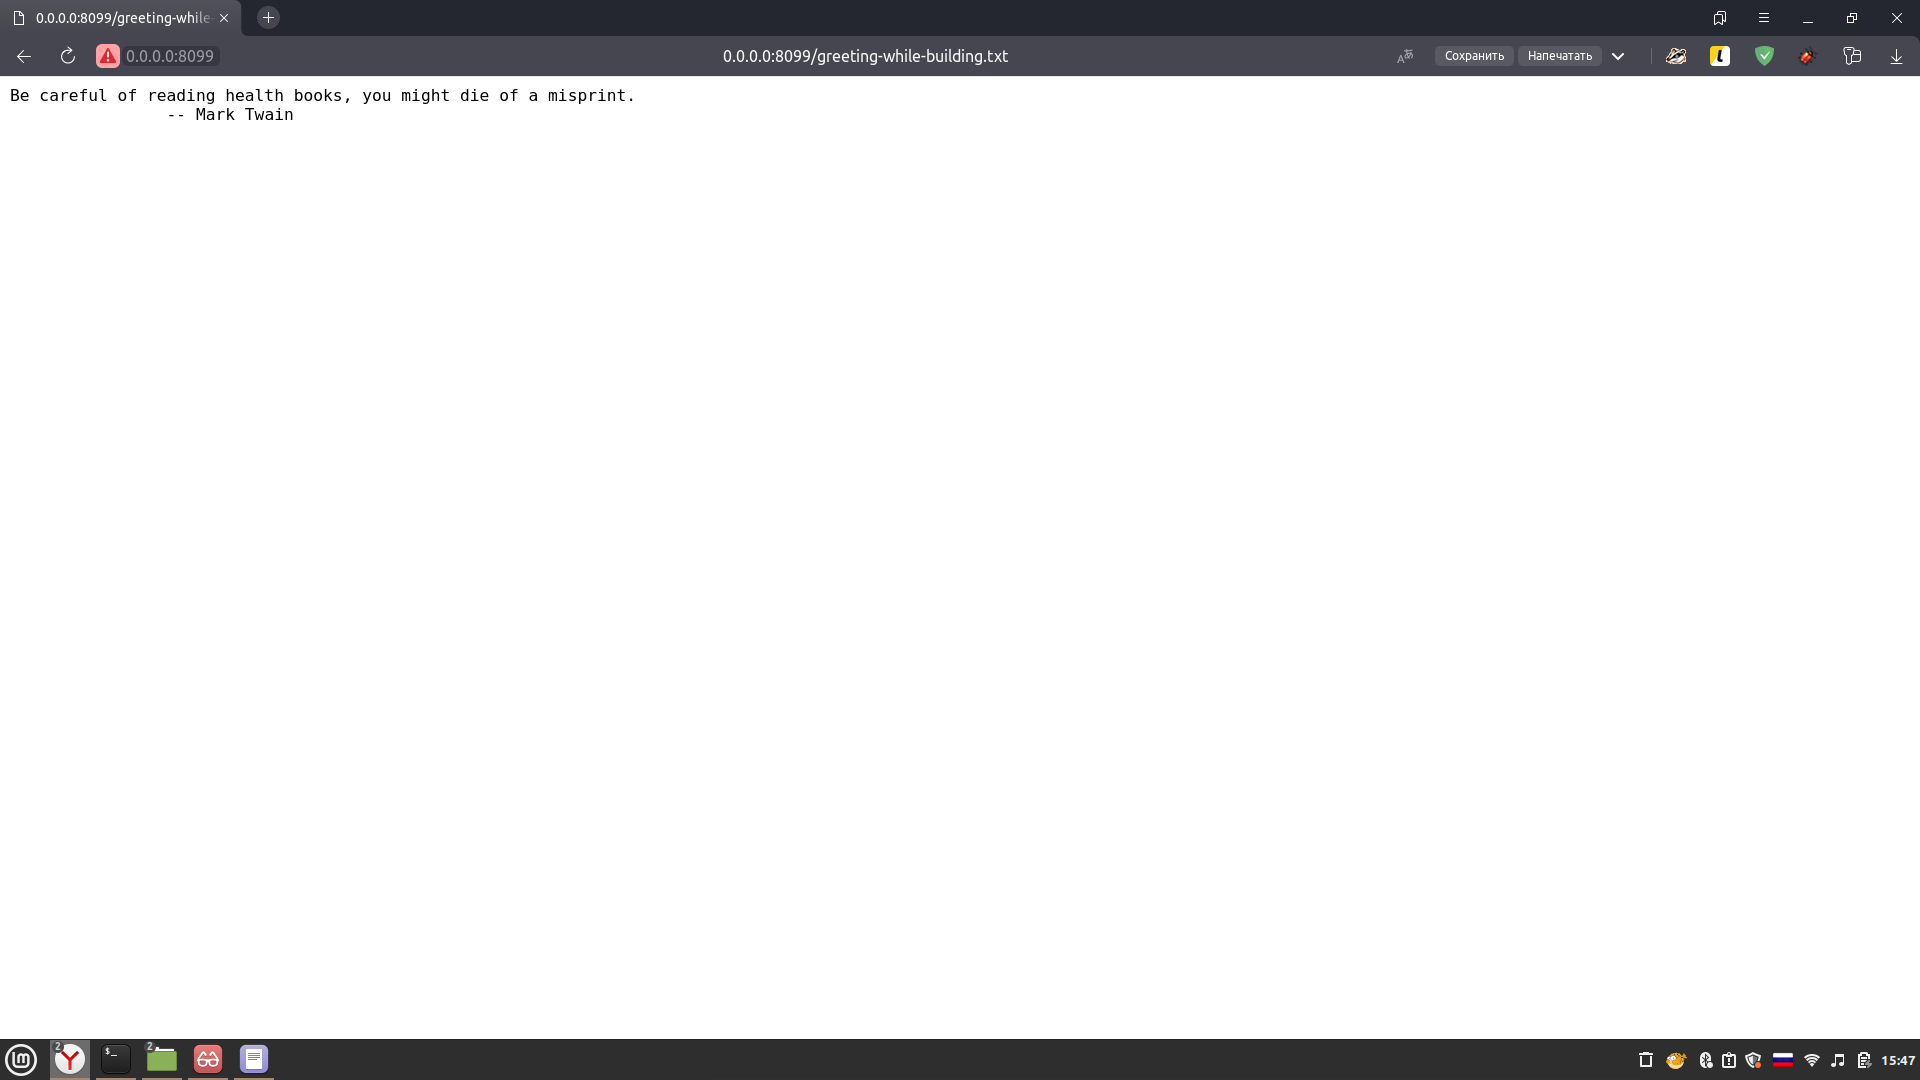
\includegraphics[width=\linewidth]{7file}
	\caption{Dockerfile. Файл}
	\label{img:7file}
\end{figure}

\begin{figure}[hptb]
	\centering
	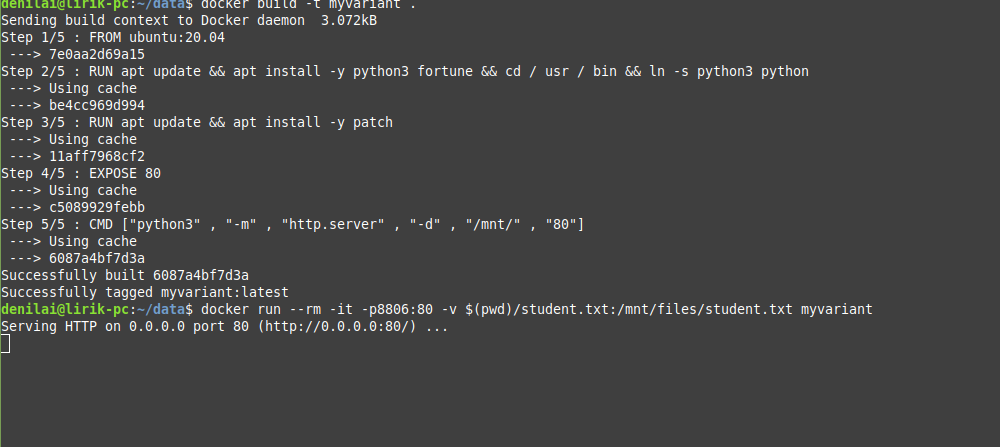
\includegraphics[width=\linewidth]{8com}
	\caption{Индивидуальное задание. Команды}
	\label{img:8com}
\end{figure}


\begin{figure}[hptb]
	\centering
	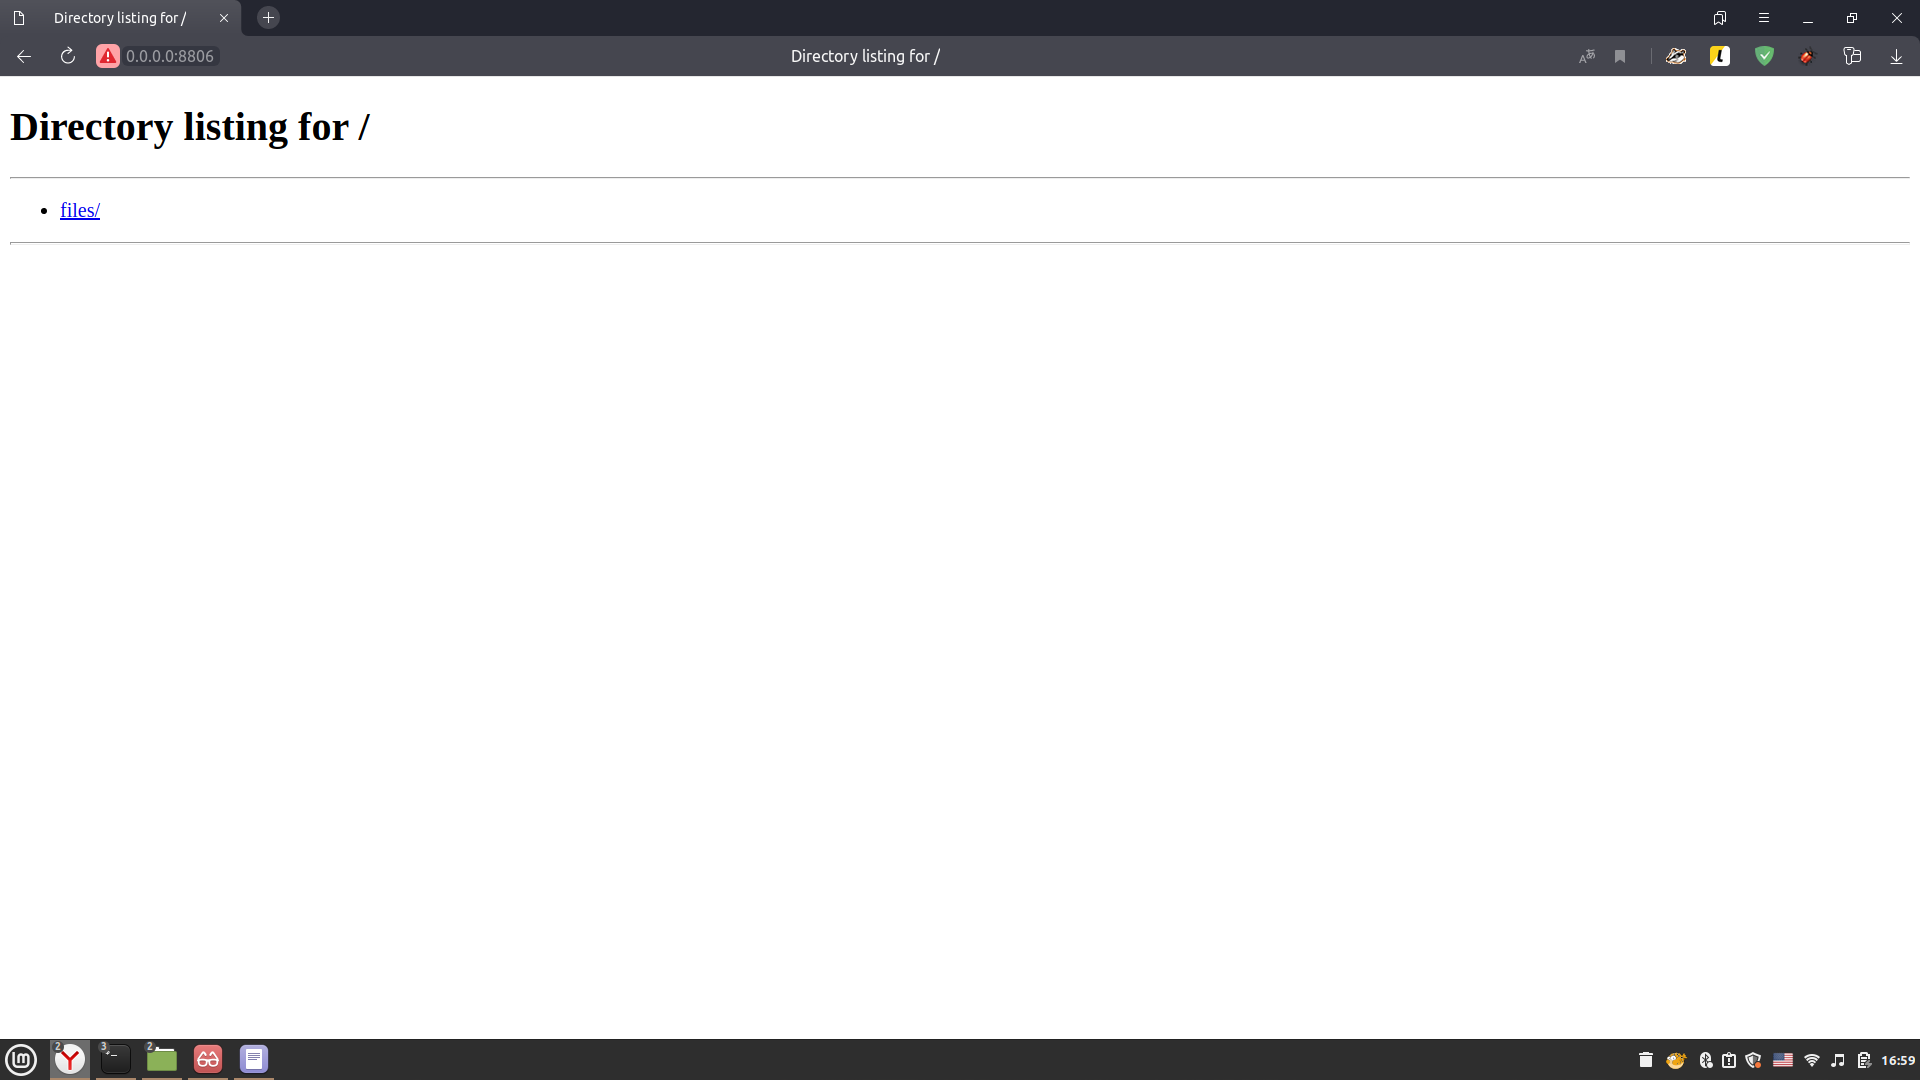
\includegraphics[width=\linewidth]{8serv}
	\caption{Индивидуальное задание. Сервер}
	\label{img:8serv}
\end{figure}
\newpage
\begin{figure}[hptb]
	\centering
	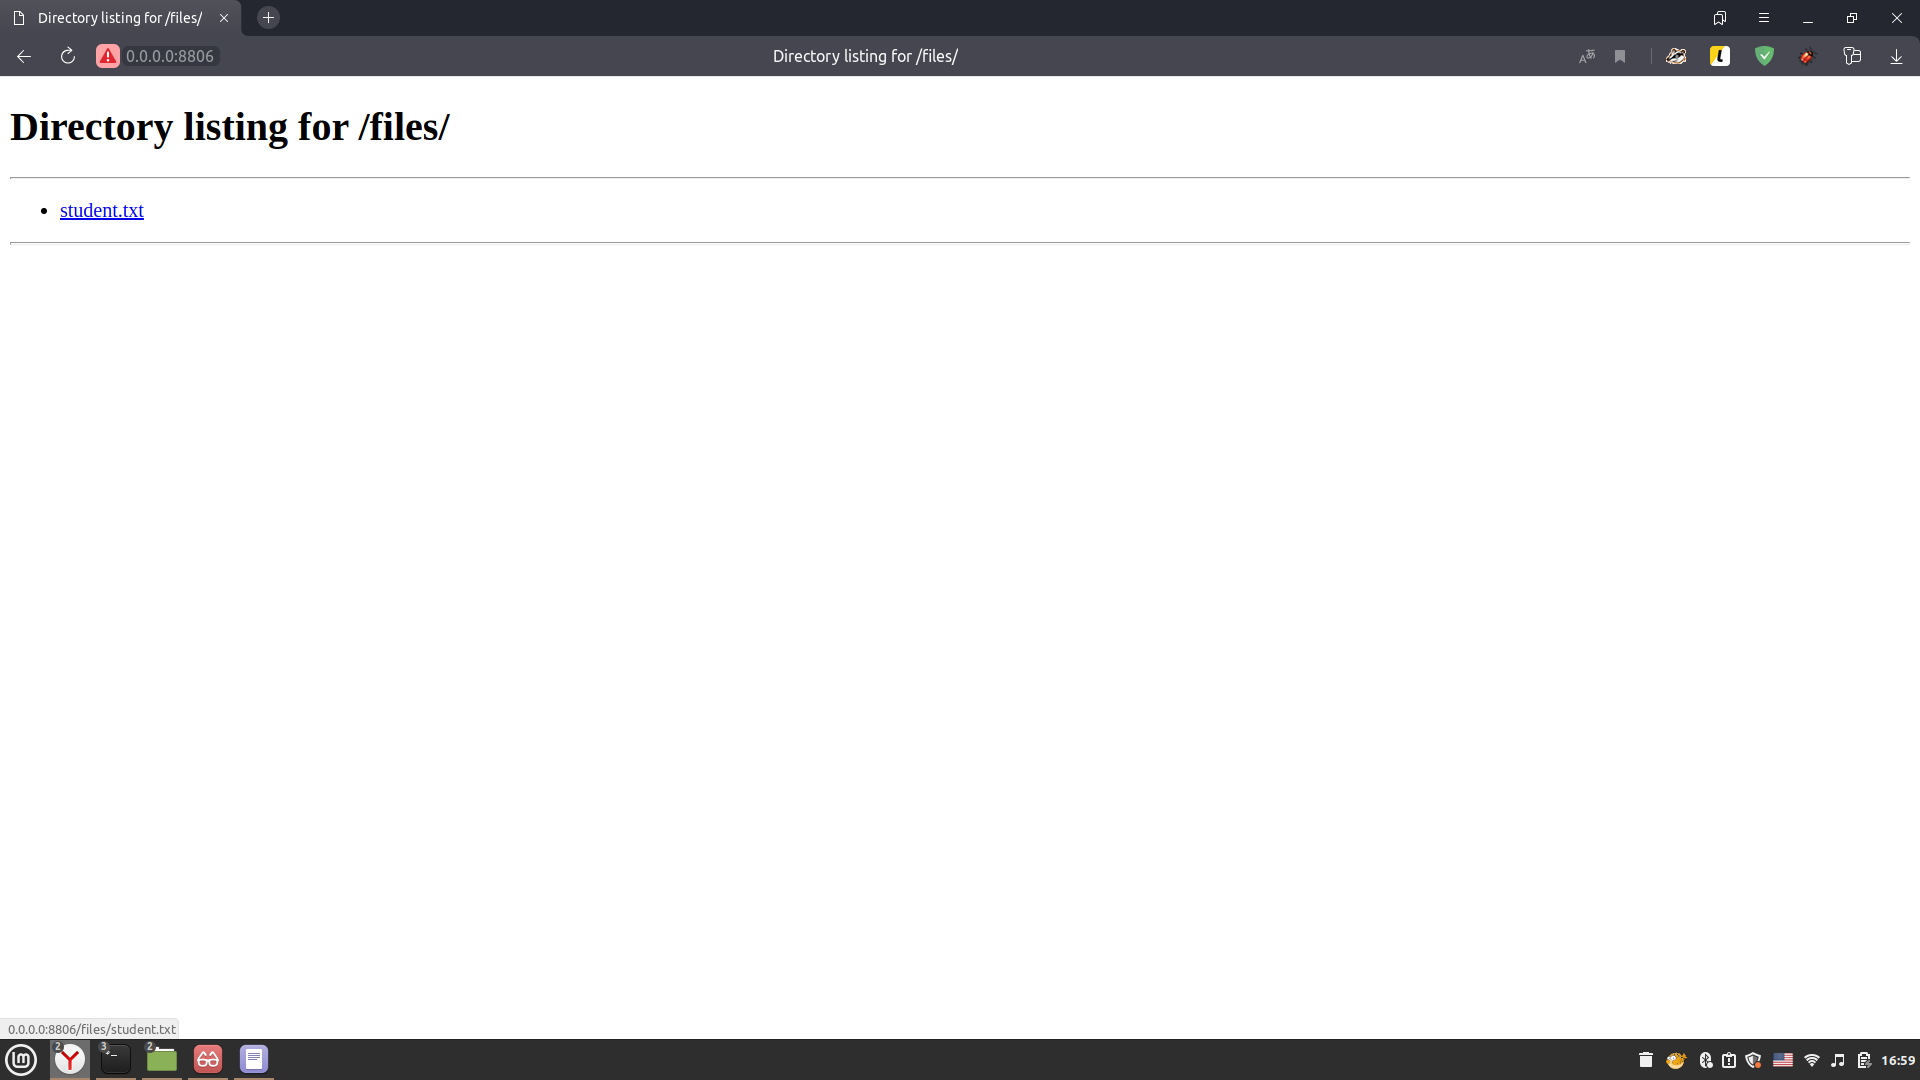
\includegraphics[width=\linewidth]{8serv1}
	\caption{Индивидуальное задание. Сервер}
	\label{img:8serv1}
\end{figure}

\newpage
\begin{figure}[hptb]
	\centering
	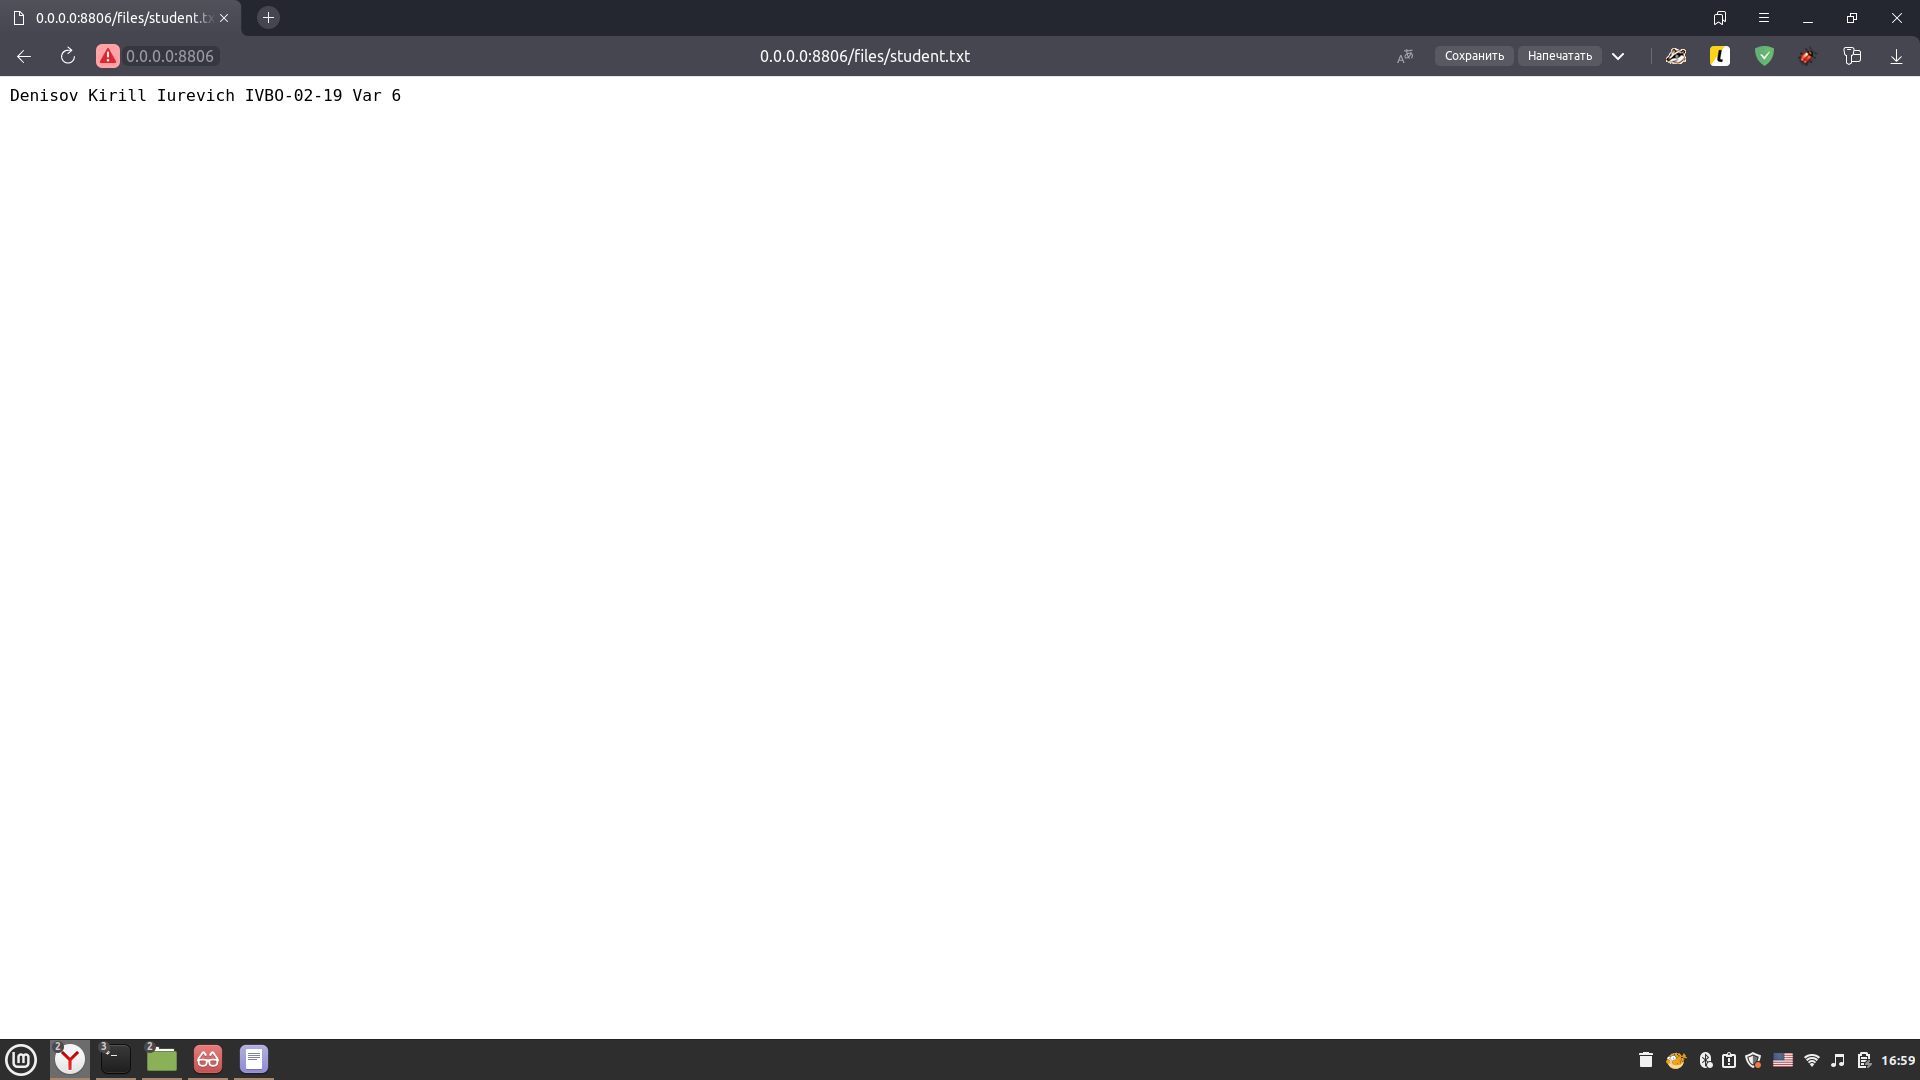
\includegraphics[width=\linewidth]{8file}
	\caption{Индивидуальное задание. Файл}
	\label{img:8file}
\end{figure}


\end{document}
